%%%%%%%%%%%%%%%%%%%%%%%%%%%%%%%%%%%%%%%%%
% Beamer Presentation
% LaTeX Template
% Version 1.0 (10/11/12)
%
% This template has been downloaded from:
% http://www.LaTeXTemplates.com
%
% License:
% CC BY-NC-SA 3.0 (http://creativecommons.org/licenses/by-nc-sa/3.0/)
%
%%%%%%%%%%%%%%%%%%%%%%%%%%%%%%%%%%%%%%%%%

%----------------------------------------------------------------------------------------
%	PACKAGES AND THEMES
%----------------------------------------------------------------------------------------

 \documentclass{beamer}

\mode<presentation> {

% The Beamer class comes with a number of default slide themes
% which change the colors and layouts of slides. Below this is a list
% of all the themes, uncomment each in turn to see what they look like.

%\usetheme{default}
%\usetheme{AnnArbor}
%\usetheme{Antibes}
%\usetheme{Bergen}
%\usetheme{Berkeley}
%\usetheme{Berlin}
%\usetheme{Boadilla}
%\usetheme{CambridgeUS}
%\usetheme{Copenhagen}
%\usetheme{Darmstadt}
%\usetheme{Dresden}
%\usetheme{Frankfurt}
%\usetheme{Goettingen}
%\usetheme{Hannover}
%\usetheme{Ilmenau}
%\usetheme{JuanLesPins}
%\usetheme{Luebeck}
\usetheme{Madrid}
%\usetheme{Malmoe}
%\usetheme{Marburg}
%\usetheme{Montpellier}
%\usetheme{PaloAlto}
%\usetheme{Pittsburgh}
%\usetheme{Rochester}
%\usetheme{Singapore}
%\usetheme{Szeged}
%\usetheme{Warsaw}

% As well as themes, the Beamer class has a number of color themes
% for any slide theme. Uncomment each of these in turn to see how it
% changes the colors of your current slide theme.

%\usecolortheme{albatross}
%\usecolortheme{beaver}
%\usecolortheme{beetle}
%\usecolortheme{crane}
%\usecolortheme{dolphin}
%\usecolortheme{dove}
%\usecolortheme{fly}
%\usecolortheme{lily}
%\usecolortheme{orchid}
%\usecolortheme{rose}
%\usecolortheme{seagull}
%\usecolortheme{seahorse}
%\usecolortheme{whale}
%\usecolortheme{wolverine}

%\setbeamertemplate{footline} % To remove the footer line in all slides uncomment this line
%\setbeamertemplate{footline}[page number] % To replace the footer line in all slides with a simple slide count uncomment this line

%\setbeamertemplate{navigation symbols}{} % To remove the navigation symbols from the bottom of all slides uncomment this line
}
\usepackage{graphicx} % Allows including images
\usepackage{booktabs} % Allows the use of \toprule, \midrule and \bottomrule in tables
\usepackage{amsmath}
\usepackage{mathrsfs}
\bibliographystyle{ieeetr}
%----------------------------------------------------------------------------------------
%	TITLE PAGE
%----------------------------------------------------------------------------------------

\title[Assignment]{Assignment: 3-Achieving Usable and Privacy-assured Similarity Search over Outsourced Cloud Data} % The short title appears at the bottom of every slide, the full title is only on the title page

\author{Xinyi Li} % Your name
\institute[DLUT] % Your institution as it will appear on the bottom of every slide, may be shorthand to save space
{
Dalian University of Technology \\
\textit{Assignment of System Security} % Your institution for the title page
\medskip % Your email address
}
\date{\today} % Date, can be changed to a custom date

\begin{document}


\begin{frame}
\titlepage % Print the title page as the first slide
\end{frame}

\begin{frame}
	\frametitle{Overview} % Table of contents slide, comment this block out to remove it
	\tableofcontents % Throughout your presentation, if you choose to use \section{} and \subsection{} commands, these will automatically be printed on this slide as an overview of your presentation
\end{frame}
\section{Introduction}
\begin{frame}
	\frametitle{Introduction of the Paper}
	\bibliography{myreference}    
\end{frame}

\begin{frame}
 \frametitle{Introduction of the Paper}
 \begin{block}{Purpose}
  Solve the problem of secure and efficient fuzzy search over encrypted outsourced cloud data
  \end{block}
  
  \begin{block}{Measures}
  	\begin{itemize}
  		\item Suppressing technique 
  		\item Building a private trie-traverse searching index
  	\end{itemize}
  \end{block}
  
  \begin{block}{Performance}
	  Correctly achieves the defined similarity search functionality with \textbf{\textcolor{red}{constant}}  searching time!
  \end{block}
  
  
\end{frame}


%----------------------------------------------------------------------------------------
%	PRESENTATION SLIDES
%----------------------------------------------------------------------------------------

%------------------------------------------------
\section{Background} % Sections can be created in order to organize your presentation into discrete blocks, all sections and subsections are automatically printed in the table of contents as an overview of the talk
%------------------------------------------------
\begin{frame}
	\frametitle{System and Threat Model}
	\begin{figure}
	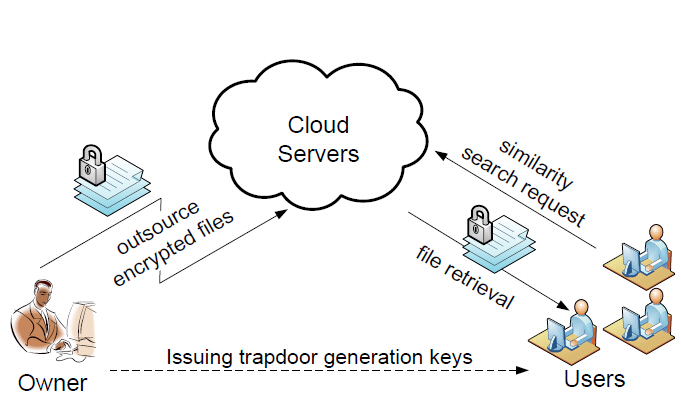
\includegraphics[width=0.6\linewidth]{fig1.jpg}
	\caption[1]{Architecture of similarity keyword search over outsourced cloud data}
	\end{figure}
		\begin{itemize}
			\item data owner: the individual/enterprise customer,who has a collection of $n$ data files $C = ({F_1},{F_2}, \ldots ,{F_n})$ to be stored in the cloud server.
			\item $W = \left\{ {{w_i},{w_w}, \ldots ,{w_p}} \right\}$ is denoted as a predefined set of distinct keywords in $C$
		\end{itemize}
\end{frame}
%\subsection{Subsection Example} % A subsection can be created just before a set of slides with a common theme to further break down your presentation into chunks
\begin{frame}
	\frametitle{System and Threat Model}
	\begin{itemize}
		\item Files are encrypted before outsourced
		\item The data owner will distribute search request\textcolor{red}{(trapdoor) generation keys $sk$} to authorized users.(Assume that the authorization will be done appropriately)
		\item An authorized user uses \textcolor{red}{trapdoor generation key} to generate a search request via some \textcolor{red}{one-way function} to search word $w$, and submit it to the cloud.
		\item The cloud then performs the search over the data
		collection $C$ without decryption and sends back all encrypted files containing the specific keyword $w$, denoted as $FI{D_w}$.
		\item \textcolor{blue} {The
		similarity keyword search scheme returns the closest possible results based on aforementioned measures.}
		\item At last, the user decrypts files they received from the cloud.
	\end{itemize}
\end{frame}

\begin{frame}
	\frametitle{Assumption: Honest-but-curious clound server}
    To ensure the securely similarity searching schema:
    \begin{columns}[t] 
    \column{.3\textwidth}
    \begin{block}{Honest}
    	Correctly follows the designated protocol specification
    \end{block}
    \column{.5\textwidth}
        \begin{alertblock}{Curious}
        	Infer and analyze the message flow received during the protocol so as to learn additional information
        \end{alertblock}
    \end{columns}
    \begin{columns}
    \column{.8\textwidth}
    \begin{exampleblock}{}
        We follow the security definition
        deployed in the traditional  \textcolor{red} {searchable symmetric encryption(SSE)}
    \end{exampleblock}
\end{columns}
\end{frame}

\begin{frame}
	\frametitle{Notations}
	\begin{description}
		\item[$C$]the file collection to be outsourced, denoted as a set of $n$ data files $C = ({F_1},{F_2}, \ldots ,{F_n})$.
		\item[$W$]the distinct keywords extracted from file collection $C$, denoted as a set of $m$ words $W = \left\{ {{w_i},{w_w}, \ldots ,{w_p}} \right\}$.
		\item[$\cal I$]the index built for privacy-assured similarity search.
		\item[${T_w}$] the trapdoor generated by a user as a search request of input keyword $w$ via some one-way transformation.
		\item[${S_{w,d}}$] similarity keyword set of $w$, where $d$ is the similarity threshold according to a certain similarity metrics.
		\item[$FI{D_{{w_i}}}$]the set of identifiers of files in $C$ that contain keyword ${{w_i}}$.
		\item[$f(key, \cdot ),g(key, \cdot )$]pseudorandom function (PRF), defined	as: ${\{ 0,1\} ^*} \times key \to {\{ 0,1\} ^{\ell }}$.
		\item[$Enc(key, \cdot ),Dec(key, \cdot )$]symmetric key based semantic secure encryption/decryption function.
	\end{description}
\end{frame}

\begin{frame}
	\frametitle{Edit Distance}
	\begin{columns}
	\end{columns}
	\begin{block}{Quantitative measurement}
		The edit distance $ed({w_1},{w_2})$ between two words ${w_1}$ and ${w_2}$ is the \textcolor{red}{mininum} number of \textcolor{red}{primitive operations}, including \textcolor{blue}{character insertion, deletion} and \textcolor{blue}{substitution}, necessary to transform one of them into the other.
	\end{block}
	
	\begin{block}{Similarity keyword set}
		Given a keyword $w$, we let ${S_{w,d}}$ denote its similarity set of words, such that any $w' \in {S_{w,d}}$ satisfies \textcolor[rgb]{0.1,0.6,0.3}{$ed(w,w') \le d$}  for a certain integer $d$.
	\end{block}
	
	\begin{exampleblock}{Example}
		Consider the keyword $w_0=$\textit{CENSOR}\\
		a words set W = \{\textit{CESOR},\textit{CENSER},\textit{CEANSOR}\}\\
		for any $w' \in W$,$ed({w_0},w') \le 1$ holds,\\
		i.e. $w' \in {S_{{w_0},1}}$ and $W \subseteq {S_{{w_0},1}}$
	\end{exampleblock}
\end{frame}

\begin{frame}
	\frametitle{Building Similarity Keyword Sets}
	\begin{columns}
		\column{.45\textwidth}
		\begin{alertblock}{Straightforward approach}
			Simply \textcolor{red}{enumerating} all possible words $w{'_i}$ satisfying the similarity
			criteria $ed({w_i},w{'_i}) \le d$
		\end{alertblock}
		\begin{alertblock}{}
		For the keyword $w_0=$\textit{CENSOR},
		consider just one substitution operation with charaters on first character.\\
		There are 26 items \{\textit{AENSOR},\textit{BENSOR}, \ldots ,\textit{YENSOR},\textit{ZENSOR}\} \\
		So ${S_{{w_0},1}}$ will be $[6 + (6 + 1)] \times \textcolor{red}{26} + \textcolor{green}1$
		\end{alertblock}
		\column{.5\textwidth}
		\begin{block}{Suppression technique}
			Consider only the \textcolor{blue}{positions} of the primitive edit operations.Specifically, we use a \textcolor{blue}{wildcard ‘*’ }to
			denote all three operations of character insertion, deletion and
			substitution at any position.
		\end{block}
		
		\begin{block}{}
			Now,\\
 ${{{S}}_{SENSOR,1}} = $ \{\textit{SENSOR}, \textit{*SENSOR, *ENSOR},\textit{S*ENSOR}, \textit{S*NSOR}, \ldots, \textit{SENSO*R}, \textit{SENSO*}, \textit{SENSOR*}\}.
			Size can be reduced to ${S_{{w_0},1}}$ will be $[6 + (6 + 1)] \times \textcolor{blue}{1} + \textcolor{green}1$
		\end{block}
	\end{columns}
\end{frame}

\begin{frame}
	\frametitle{Building Similarity Keyword Sets}
	\begin{figure}
		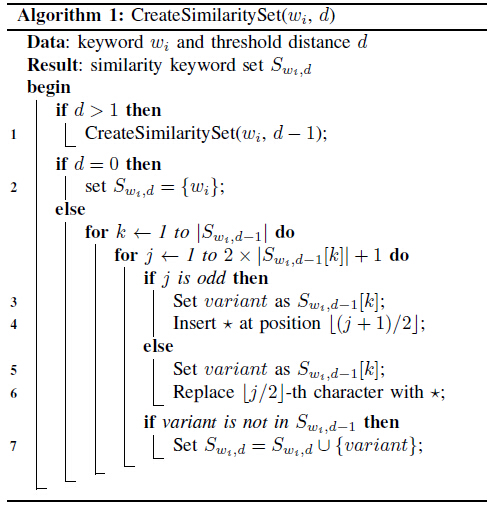
\includegraphics[width=0.4\linewidth]{algo1.jpg}
	\end{figure}
	The size of ${S_{{w_i},d}}$ will be ${\cal O}(\textcolor{blue}{\ell ^d})$,opposing to ${\cal O}(\textcolor{blue}{{\ell ^d}} \times \textcolor{red}{26^d})$ obtained in the \textcolor{red}{straightforward approach}.
\end{frame}

\begin{frame}
	\frametitle{Generating Searching Request}
	\begin{theorem}
		The intersection of the similarity sets ${S_{{w_i},d}}$ and ${S_{w,d}}$ for keyword $w_i$ and  search input $w$ is not empty if and only if $ed(w,{w_i}) \le d$.
	\end{theorem}
	
	\begin{proof}
		\begin{itemize}
			\item Completeness(i.e. $ed(w,{w_i}) \le d \to {S_{{w_i},d}} \cap {S_{w,d}} \ne \emptyset $ ):
			\begin{itemize}
				\item $\textcolor{red}{w} \to \textcolor{blue}{{w_i}}$ need at most $d$ primitive operations.
				\item \textcolor{red}{$w$} must be in \textcolor{blue}{${S_{{w_i},d}}$} 
				\item \textcolor{red}{$w$} is naturally in \textcolor{red}{${S_{w,d}}$}
			\end{itemize}
		\end{itemize}
	\end{proof}
\end{frame}

\begin{frame}
	\frametitle{Generating Searching Request}
	\begin{proof}
		\begin{itemize}
			\item Soundness(i.e. ${S_{{w_i},d}} \cap {S_{w,d}} \ne \emptyset  \to ed(w,{w_i}) \le d$) \\
			\begin{description}
				\item[${w^*}$]the common element in ${S_{{w_i},d}} \cap {S_{w,d}}$
			\end{description}
			\begin{enumerate}
				\item ${w^*}$ does not contain any wildcard *,\\
				then ${w^*} =\textcolor{red}{ w} =\textcolor{blue}{ w'}$,and $ed(\textcolor{red}{w},\textcolor{blue}{w'}) = 0 \le d$
				\item ${w^*}$ does contain some wildcard *(at most d *'s),\\
				change * in $w^*$ back to the character in \textcolor{red}{$w$} and \textcolor{blue}{$w_i$},\\
				denote the result as \textcolor{red}{$w{'^*}$} and \textcolor{blue}{$w{'_i}^*$} with both sharing $d-1$ different *'s.\\
				$\textcolor{red}{w{'^*}} \to \textcolor{blue}{w{'_i}^*}$ need at most one primitive operation.\\
				So, $ed(\textcolor{red}{w{'^*}},\textcolor{blue}{w{'_i}^*}) \le 1$\\
				$ \Rightarrow ed(\textcolor{red}{w},\textcolor{blue}{{w_i}}) \le d$
				
			\end{enumerate}
		\end{itemize}
	\end{proof}
\end{frame}
\begin{frame}
\frametitle{Paragraphs of Text}
Sed iaculis dapibus gravida. Morbi sed tortor erat, nec interdum arcu. Sed id lorem lectus. Quisque viverra augue id sem ornare non aliquam nibh tristique. Aenean in ligula nisl. Nulla sed tellus ipsum. Donec vestibulum ligula non lorem vulputate fermentum accumsan neque mollis.\\~\\

Sed diam enim, sagittis nec condimentum sit amet, ullamcorper sit amet libero. Aliquam vel dui orci, a porta odio. Nullam id suscipit ipsum. Aenean lobortis commodo sem, ut commodo leo gravida vitae. Pellentesque vehicula ante iaculis arcu pretium rutrum eget sit amet purus. Integer ornare nulla quis neque ultrices lobortis. Vestibulum ultrices tincidunt libero, quis commodo erat ullamcorper id.
\end{frame}

%------------------------------------------------

\begin{frame}
\frametitle{Bullet Points}
\begin{itemize}
\item Lorem ipsum dolor sit amet, consectetur adipiscing elit
\item Aliquam blandit faucibus nisi, sit amet dapibus enim tempus eu
\item Nulla commodo, erat quis gravida posuere, elit lacus lobortis est, quis porttitor odio mauris at libero
\item Nam cursus est eget velit posuere pellentesque
\item Vestibulum faucibus velit a augue condimentum quis convallis nulla gravida
\end{itemize}
\end{frame}

%------------------------------------------------

\begin{frame}
\frametitle{Blocks of Highlighted Text}
\begin{block}{Block 1}
Lorem ipsum dolor sit amet, consectetur adipiscing elit. Integer lectus nisl, ultricies in feugiat rutrum, porttitor sit amet augue. Aliquam ut tortor mauris. Sed volutpat ante purus, quis accumsan dolor.
\end{block}

\begin{block}{Block 2}
Pellentesque sed tellus purus. Class aptent taciti sociosqu ad litora torquent per conubia nostra, per inceptos himenaeos. Vestibulum quis magna at risus dictum tempor eu vitae velit.
\end{block}

\begin{block}{Block 3}
Suspendisse tincidunt sagittis gravida. Curabitur condimentum, enim sed venenatis rutrum, ipsum neque consectetur orci, sed blandit justo nisi ac lacus.
\end{block}
\end{frame}

%------------------------------------------------

\begin{frame}
\frametitle{Multiple Columns}
\begin{columns}[c] % The "c" option specifies centered vertical alignment while the "t" option is used for top vertical alignment

\column{.45\textwidth} % Left column and width
\textbf{Heading}
\begin{enumerate}
\item Statement
\item Explanation
\item Example
\end{enumerate}

\column{.5\textwidth} % Right column and width
Lorem ipsum dolor sit amet, consectetur adipiscing elit. Integer lectus nisl, ultricies in feugiat rutrum, porttitor sit amet augue. Aliquam ut tortor mauris. Sed volutpat ante purus, quis accumsan dolor.

\end{columns}
\end{frame}

%------------------------------------------------
\section{Second Section}
%------------------------------------------------

\begin{frame}
\frametitle{Table}
\begin{table}
\begin{tabular}{l l l}
\toprule
\textbf{Treatments} & \textbf{Response 1} & \textbf{Response 2}\\
\midrule
Treatment 1 & 0.0003262 & 0.562 \\
Treatment 2 & 0.0015681 & 0.910 \\
Treatment 3 & 0.0009271 & 0.296 \\
\bottomrule
\end{tabular}
\caption{Table caption}
\end{table}
\end{frame}

%------------------------------------------------

\begin{frame}
\frametitle{Theorem}
\begin{theorem}[Mass--energy equivalence]
$E = mc^2$
\end{theorem}
\end{frame}

%------------------------------------------------

\begin{frame}[fragile] % Need to use the fragile option when verbatim is used in the slide
\frametitle{Verbatim}
\begin{example}[Theorem Slide Code]
\begin{verbatim}
\begin{frame}
\frametitle{Theorem}
\begin{theorem}[Mass--energy equivalence]
$E = mc^2$
\end{theorem}
\end{frame}\end{verbatim}
\end{example}
\end{frame}

%------------------------------------------------

\begin{frame}
\frametitle{Figure}
Uncomment the code on this slide to include your own image from the same directory as the template .TeX file.
%\begin{figure}
%\includegraphics[width=0.8\linewidth]{test}
%\end{figure}
\end{frame}

%------------------------------------------------

\begin{frame}[fragile] % Need to use the fragile option when verbatim is used in the slide
\frametitle{Citation}
An example of the \verb|\cite| command to cite within the presentation:\\~

This statement requires citation \cite{p1}.
\end{frame}

%------------------------------------------------

\begin{frame}
\frametitle{References}
\footnotesize{
\begin{thebibliography}{99} % Beamer does not support BibTeX so references must be inserted manually as below
\bibitem[Smith, 2012]{p1} John Smith (2012)
\newblock Title of the publication
\newblock \emph{Journal Name} 12(3), 45 -- 678.
\end{thebibliography}
}
\end{frame}

%------------------------------------------------

\begin{frame}
\Huge{\centerline{The End}}
\end{frame}

%----------------------------------------------------------------------------------------

\end{document} 